%%%%%%%%%%%%%%%%%%%%%%%%%%%%%%%%%%%%%%%%%%%%%%%%%%%%%%%%%%%%%%%%%%%%%%%%%%%
%                                                                         %
%                      ENERGY SCALE AND RANGES                            %
%                                                                         %
%%%%%%%%%%%%%%%%%%%%%%%%%%%%%%%%%%%%%%%%%%%%%%%%%%%%%%%%%%%%%%%%%%%%%%%%%%%
%% Simulation Caption Commands

% Content
The theoretical basis for the difference in energy deposition lies in the different mechanisms between charged particle interactions and photon interactions in matter.
For photons with energies between approximately \SI{0.5}{\MeV} and \SI{5}{\MeV} Compton scattering is the predominant interaction mechanism between the material and the photon.
The probability of an electron having a given kinetic energy after scattering can be expressed as \eqref{eqn:dSdEKleinNishina} (see \autoref{chap:ComptonScatter} for derivation details)
\begin{align}
  \label{eqn:dSdEKleinNishina}
\frac{d\sigma}{dE_e} = 2\pi r_e^2 \sin \theta f(\theta)\left [ \frac{1+\frac{E}{m_e c^2}\left(1-\cos\theta \right)^2}{E^2 \sin \theta} \right ]
\end{align}
provided  $f(\theta)$ is defined as $f(\theta) = \frac{1}{2}\left(\frac{E'}{E}\right)^2 \left(\frac{E'}{E} + \frac{E}{E'}-\sin^2\theta\right)$.
This distribution is shown for \iso[60]{Co} in \autoref{fig:Co60ComptonScatterSpectra}.
It is then highly likely that the Compton scattered electron will have an energy close to that of the maximum energy for the Compton scattering, \SI{0.96}{\MeV} for the \SI{1.173}{\MeV} photon and \SI{1.12}{\MeV} for the \SI{1.33}{\MeV} photon.
\begin{table}
	\caption[Characteristic Energies of Compton Scattered Electrons from Co-60]{Characteristic kinetic energies of the electrons from a Compton scattering of the two photons from \iso[60]{Co}. It is very likely that an electron will have a kinetic energy greater than \SI{0.8}{\MeV}, which has a range of \SI{0.34}{\gram\per\cm\squared} in polystyrene}.
	\label{tab:ComptonEnergiesCo60}
	\begin{tabular}{ m{4cm} m{3cm} m{3cm} m{3cm}}
	\toprule
	Gamma Energy & Mean Electron Energy & Median Electron Energy & Maximum Electron Energy \\
	\midrule
	\SI{1.17}{\MeV} & \SI{0.68}{\MeV} & \SI{0.82}{\MeV} & \SI{0.96}{\MeV} \\
	\SI{1.33}{\MeV} & \SI{0.80}{\MeV} & \SI{0.96}{\MeV} & \SI{1.12}{\MeV} \\
	Average & \SI{0.74}{\MeV} & \SI{0.89}{\MeV} &  \\
	\bottomrule
	\end{tabular}
\end{table}
\begin{figure}
  \centering
    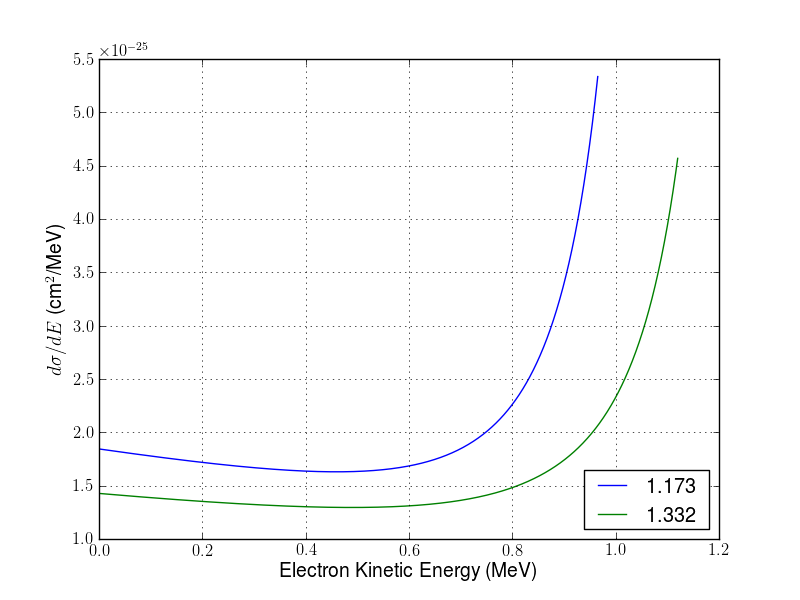
\includegraphics[width=\textwidth]{Co60ComptonScatteredSpectra}
    \caption[Analytical Co-60 Compton Electron Differential Microscopic Cross Section]{Co-60 Compton Electron Differential Microscopic Cross Section. The relative probabilities of a Compton Scattered Electron having a given kinetic energy from \iso[60]{Co} can be determined by their relative differential microscopic cross sections. For example, it almost two and a half times more likely that a Compton scattered electron will have a kinetic energy of \SI{0.95}{\MeV} than \SI{0.75}{\MeV}.}
    \label{fig:Co60ComptonScatterSpectra}
  \end{figure}
\begin{figure}
    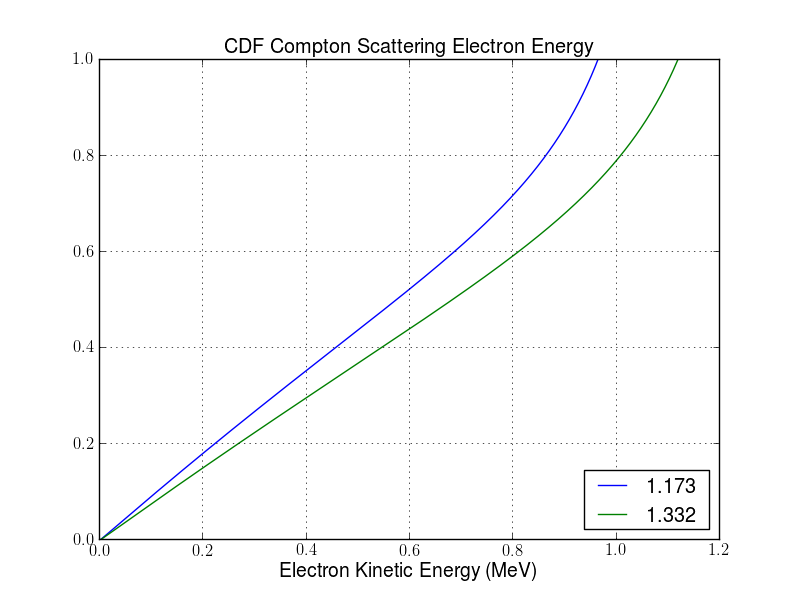
\includegraphics[width=\textwidth]{Co60ComptonScatteredSpectraCDF}
    \caption[Analytical Co-60 Compton Electron Kinetic Energy Cumulative Distribution]{Probability of the energy of a Compton Scattered Electron from \iso[60]{Co}. Over half of the electrons from the Compton scattering will have an energy greater than \SI{0.5}{\MeV}}
    \label{fig:Co60ComptonScatterCDF}
\end{figure}
The cumulative distribution function (CDF) is shown in \autoref{fig:Co60ComptonScatterCDF}.
In the case of $\iso[6]{Li}\left(n,\iso[3]{H}\right)\alpha$ the fission energy is distributed between a triton of energy \SI{2.73}{\mega\eV} and an alpha of energy \SI{2.05}{\mega\eV}.
The maximum kinetic energy of an electron from a Compton scattering event with an impingement \iso[60]{Co} source is \SI{1.117}{\mega\eV} (for the \SI{1.332}{\mega\eV} gamma). 
In polystyrene with a density of \SI{1}{\gram\per\cm\cubed}, the range of the maximum electron from Compton scattering is around \SI{4.5E3}{\um}\cite{berger_estar_2005}.
If elastic scattering between the alpha, triton and electrons is assumed the maximum kinetic energy of an electron is \SI{1.097}{\kilo\eV} for the alpha particle and \SI{1.986}{\kilo\eV} for the triton\cite{turner_atoms_2008}.
The range of the electron from a gamma interaction is more than \num{1E3} times greater than the range of electrons from an alpha or triton (\autoref{tab:BasicEDepOutline}).
Therefore, it is more likely that the electrons generated by the alpha and the triton deposit significantly more of their energy in a thin film than the electron from a gamma.
This is also reflected in the stopping power, where the reaction product secondary electrons have a stopping power 40 times that of the secondary electrons from a gamma \cite{berger_estar_2005}.
The simulated electron range distributions for several energies is shown in \autoref{fig:ElectronRangesDist} and summarized in \autoref{fig:ElectronRanges}.
The electrons  from Compton scattering of \iso[60]{Co} will be on the order of \SI{100}{\keV} , with ranges two orders of magnitude than that of electrons from the charged particle interactions.
\begin{table}[ht]
  \caption[Electron Energy, Range, and Stopping Power]{Electron Energy, Range, and Stopping Power \protect\cite{berger_estar_2005,turner_atoms_2008}}
	\centering
	\begin{tabular}{c | c S}
	\toprule
	{Electron Parent} & {Electron Energy} & {Total Stopping Power} \\
	 &  & \si{\mega\eV \cm\squared \per \gram} \\
	\midrule
	{gamma}  & \SI{1.12}{\mega\eV} & 1.79 \\
	{triton} & \SI{1.99}{\kilo\eV} & 75.1 \\
	{alpha}  & \SI{1.10}{\kilo\eV} & 113  \\
	\bottomrule
	\end{tabular}
  \label{tab:BasicEDepOutline}
	% See pg. 87 of Matthew's lab notebook for the calculation
\end{table}
\begin{figure}
  \centering
      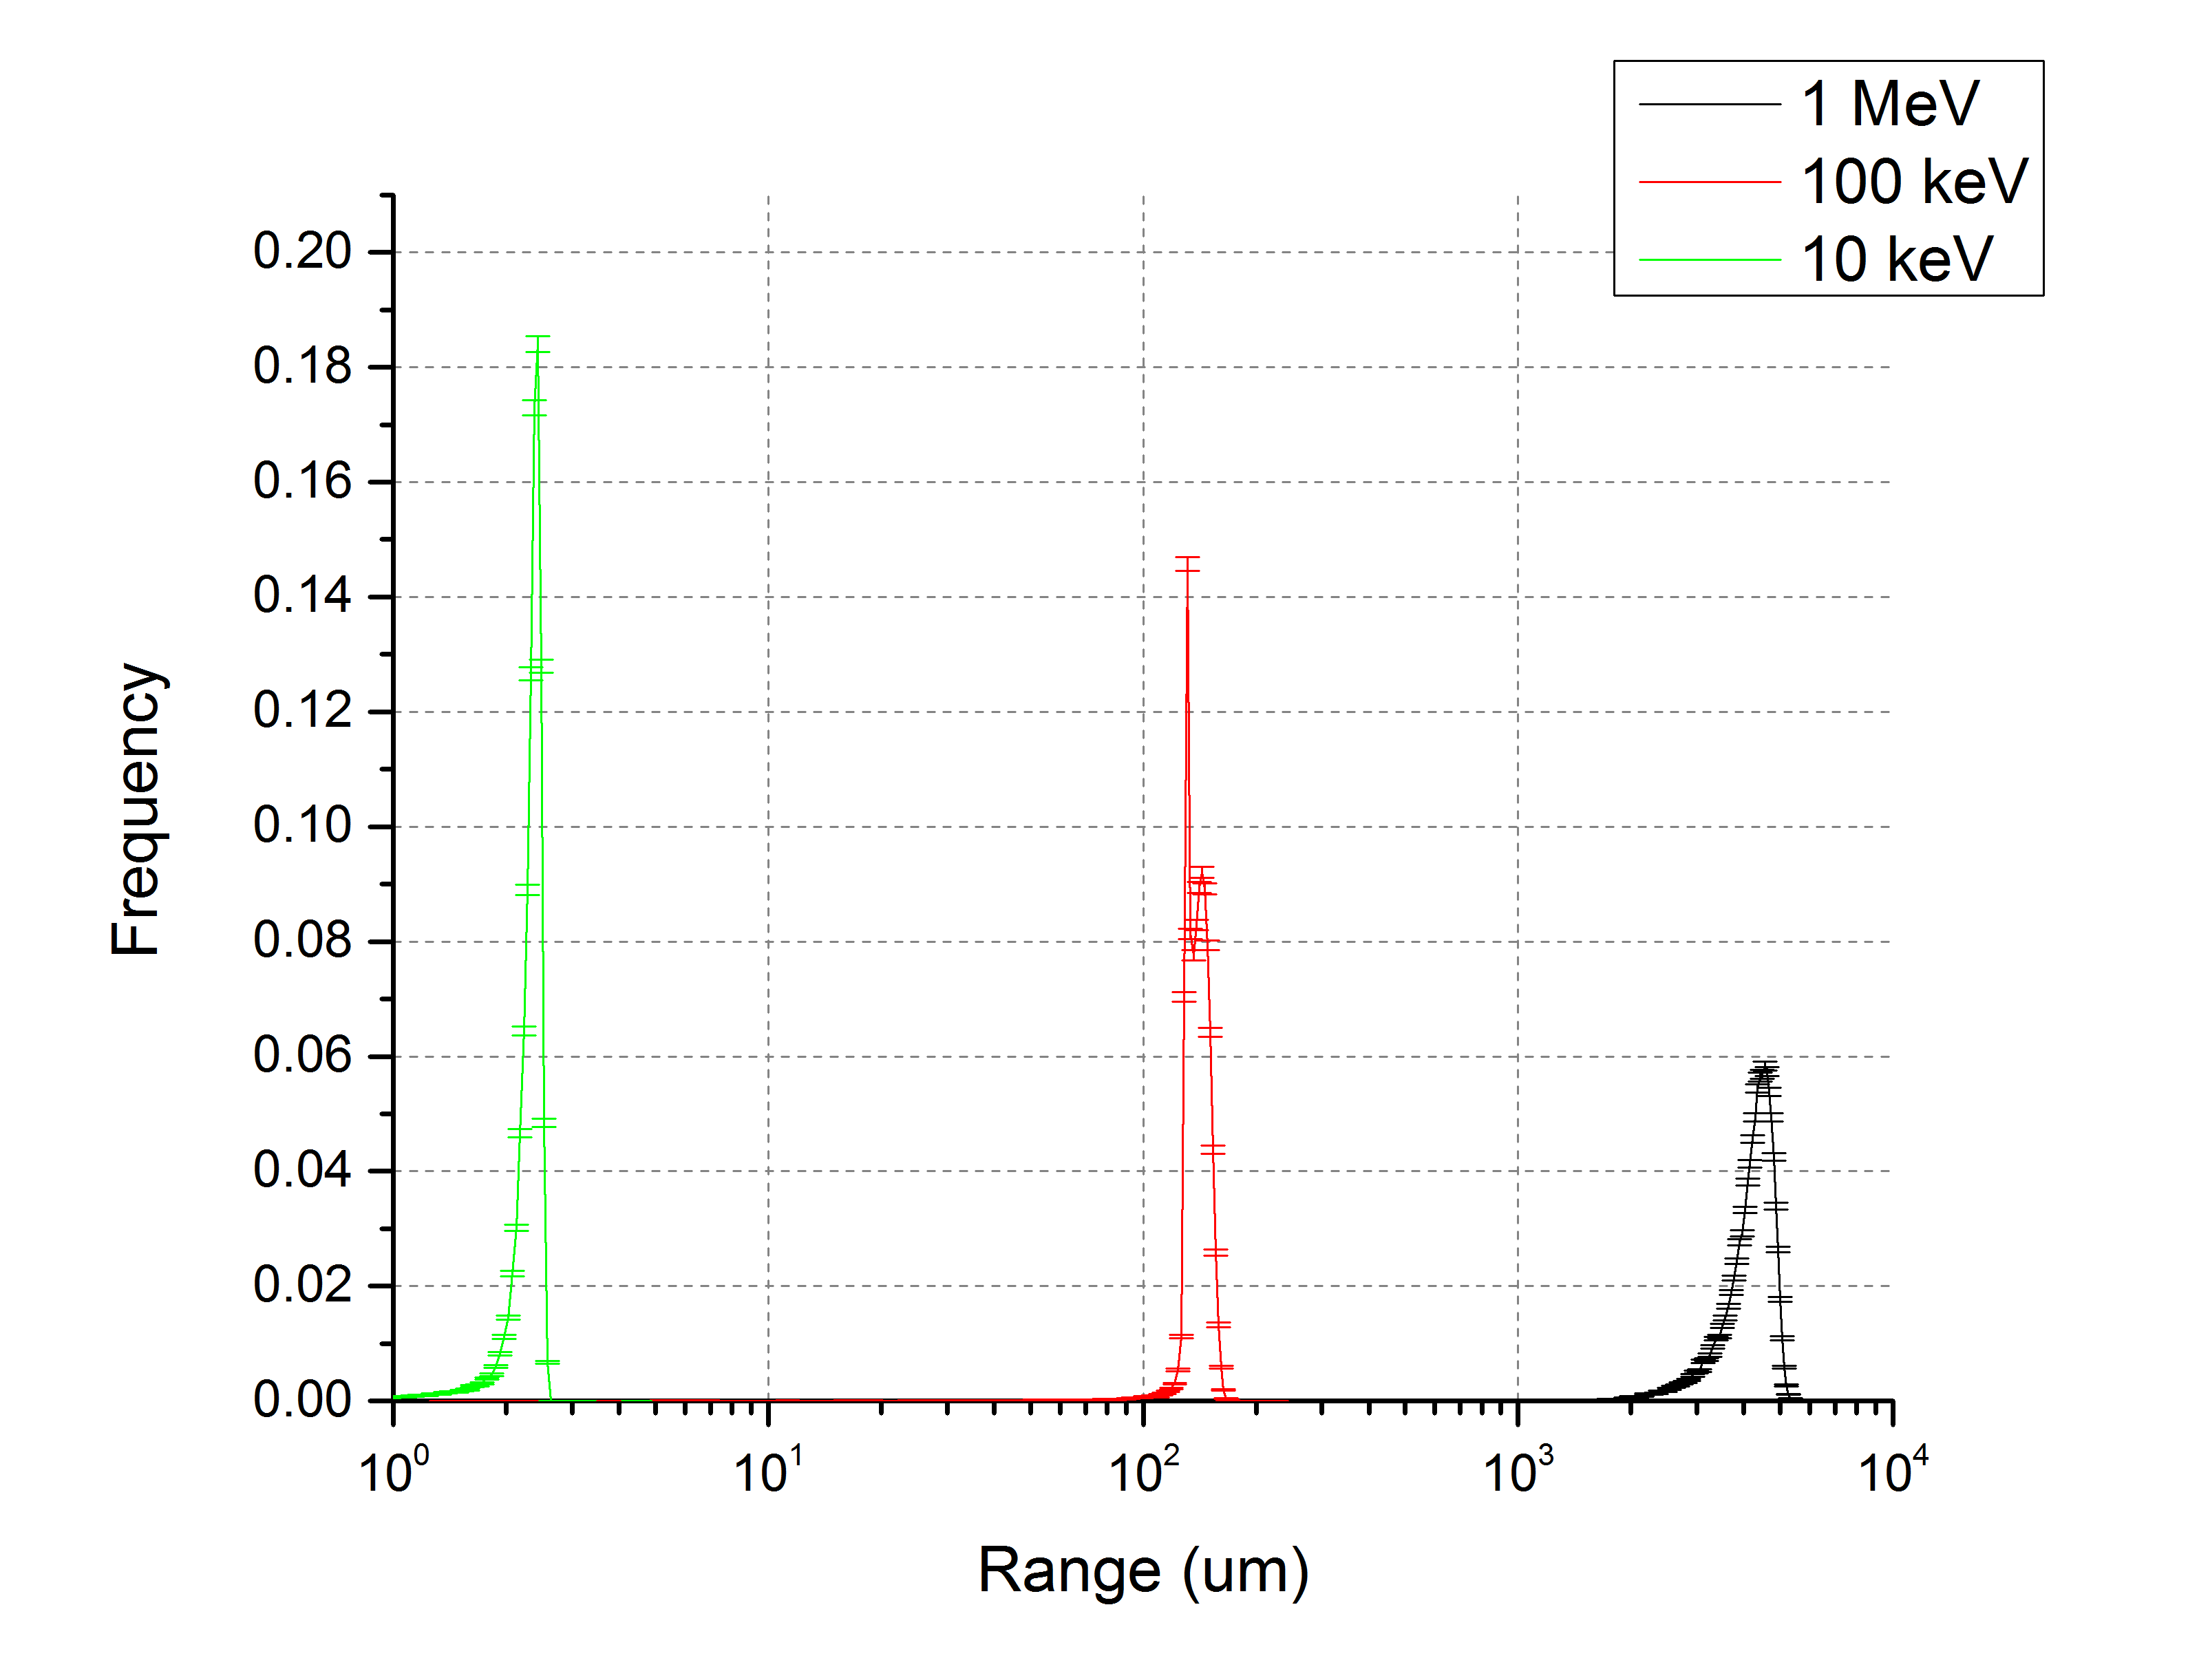
\includegraphics[width=\textwidth]{ElectronRangeDistribution}
      \caption[Simulated Electron Ranges Distributions in Polystyrene]{Simulated range of \SI{1}{\MeV}, \SI{100}{\keV}, and \SI{10}{\keV} electrons.\rangeSimGeo}
      \label{fig:ElectronRangesDist}
\end{figure}
\begin{figure}
	\centering
      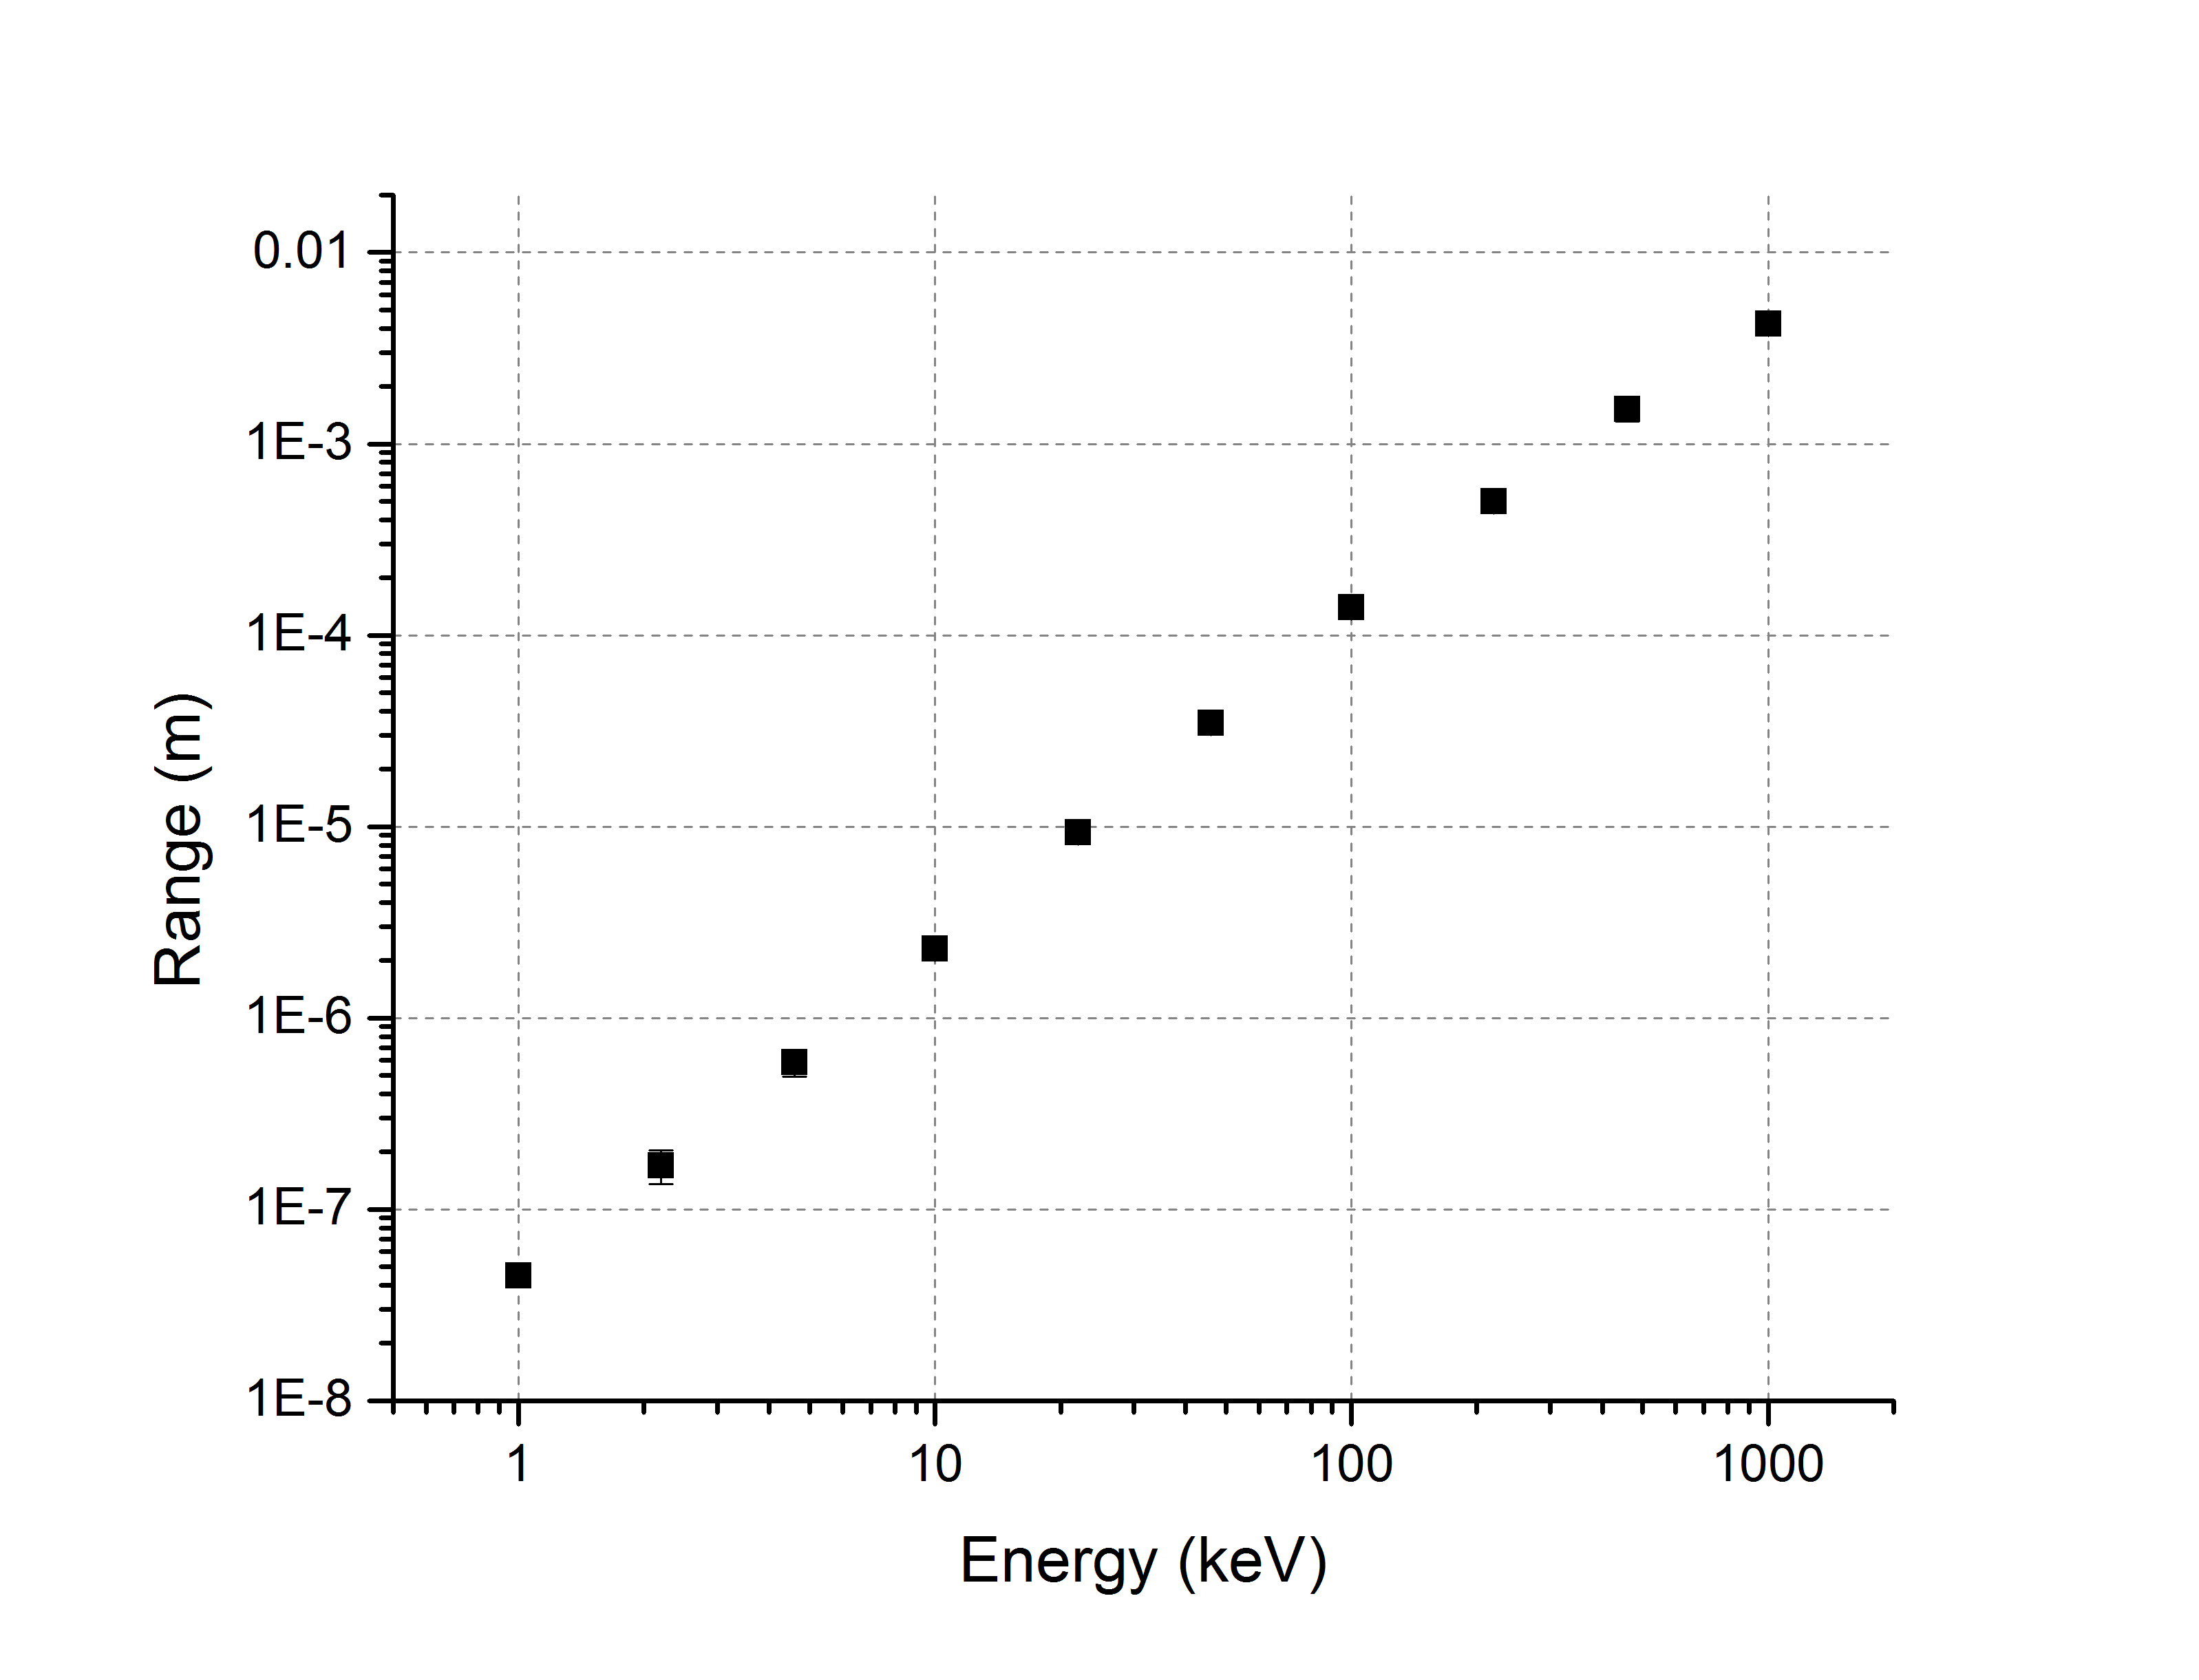
\includegraphics[width=\textwidth]{ElectronRange}
  \caption[Simulated Electron Ranges in Polystyrene]{Simulated electron ranges for electron kinetic energies ranging from \SI{1}{\keV} to \SI{1}{\MeV}.\rangeSimGeo} 
  \label{fig:ElectronRanges}
\end{figure}

The development of the secondary electron energy ranges so far has been from a simplified treatment of the problem when only the dominant process are considered.
Detailed simulations are necessary in order to have a greater understanding of the problem. 
The energy of the electrons created from an alpha (\SI{2.05}{\MeV}), triton (\SI{2.73}{\MeV}), and gammas from \iso[60]{Co} were calculated using a GEANT4 simulation, and overlaid on the range of electrons (left axis) as shown in \autoref{fig:ERangeAndDist}.
It is then clear that the electrons from the \iso[60]{Co} will travel much father than those from the $\iso[6]{Li}\left(n,\alpha\right)\iso[3]{H}$ reaction products.
\begin{figure}
  \centering
  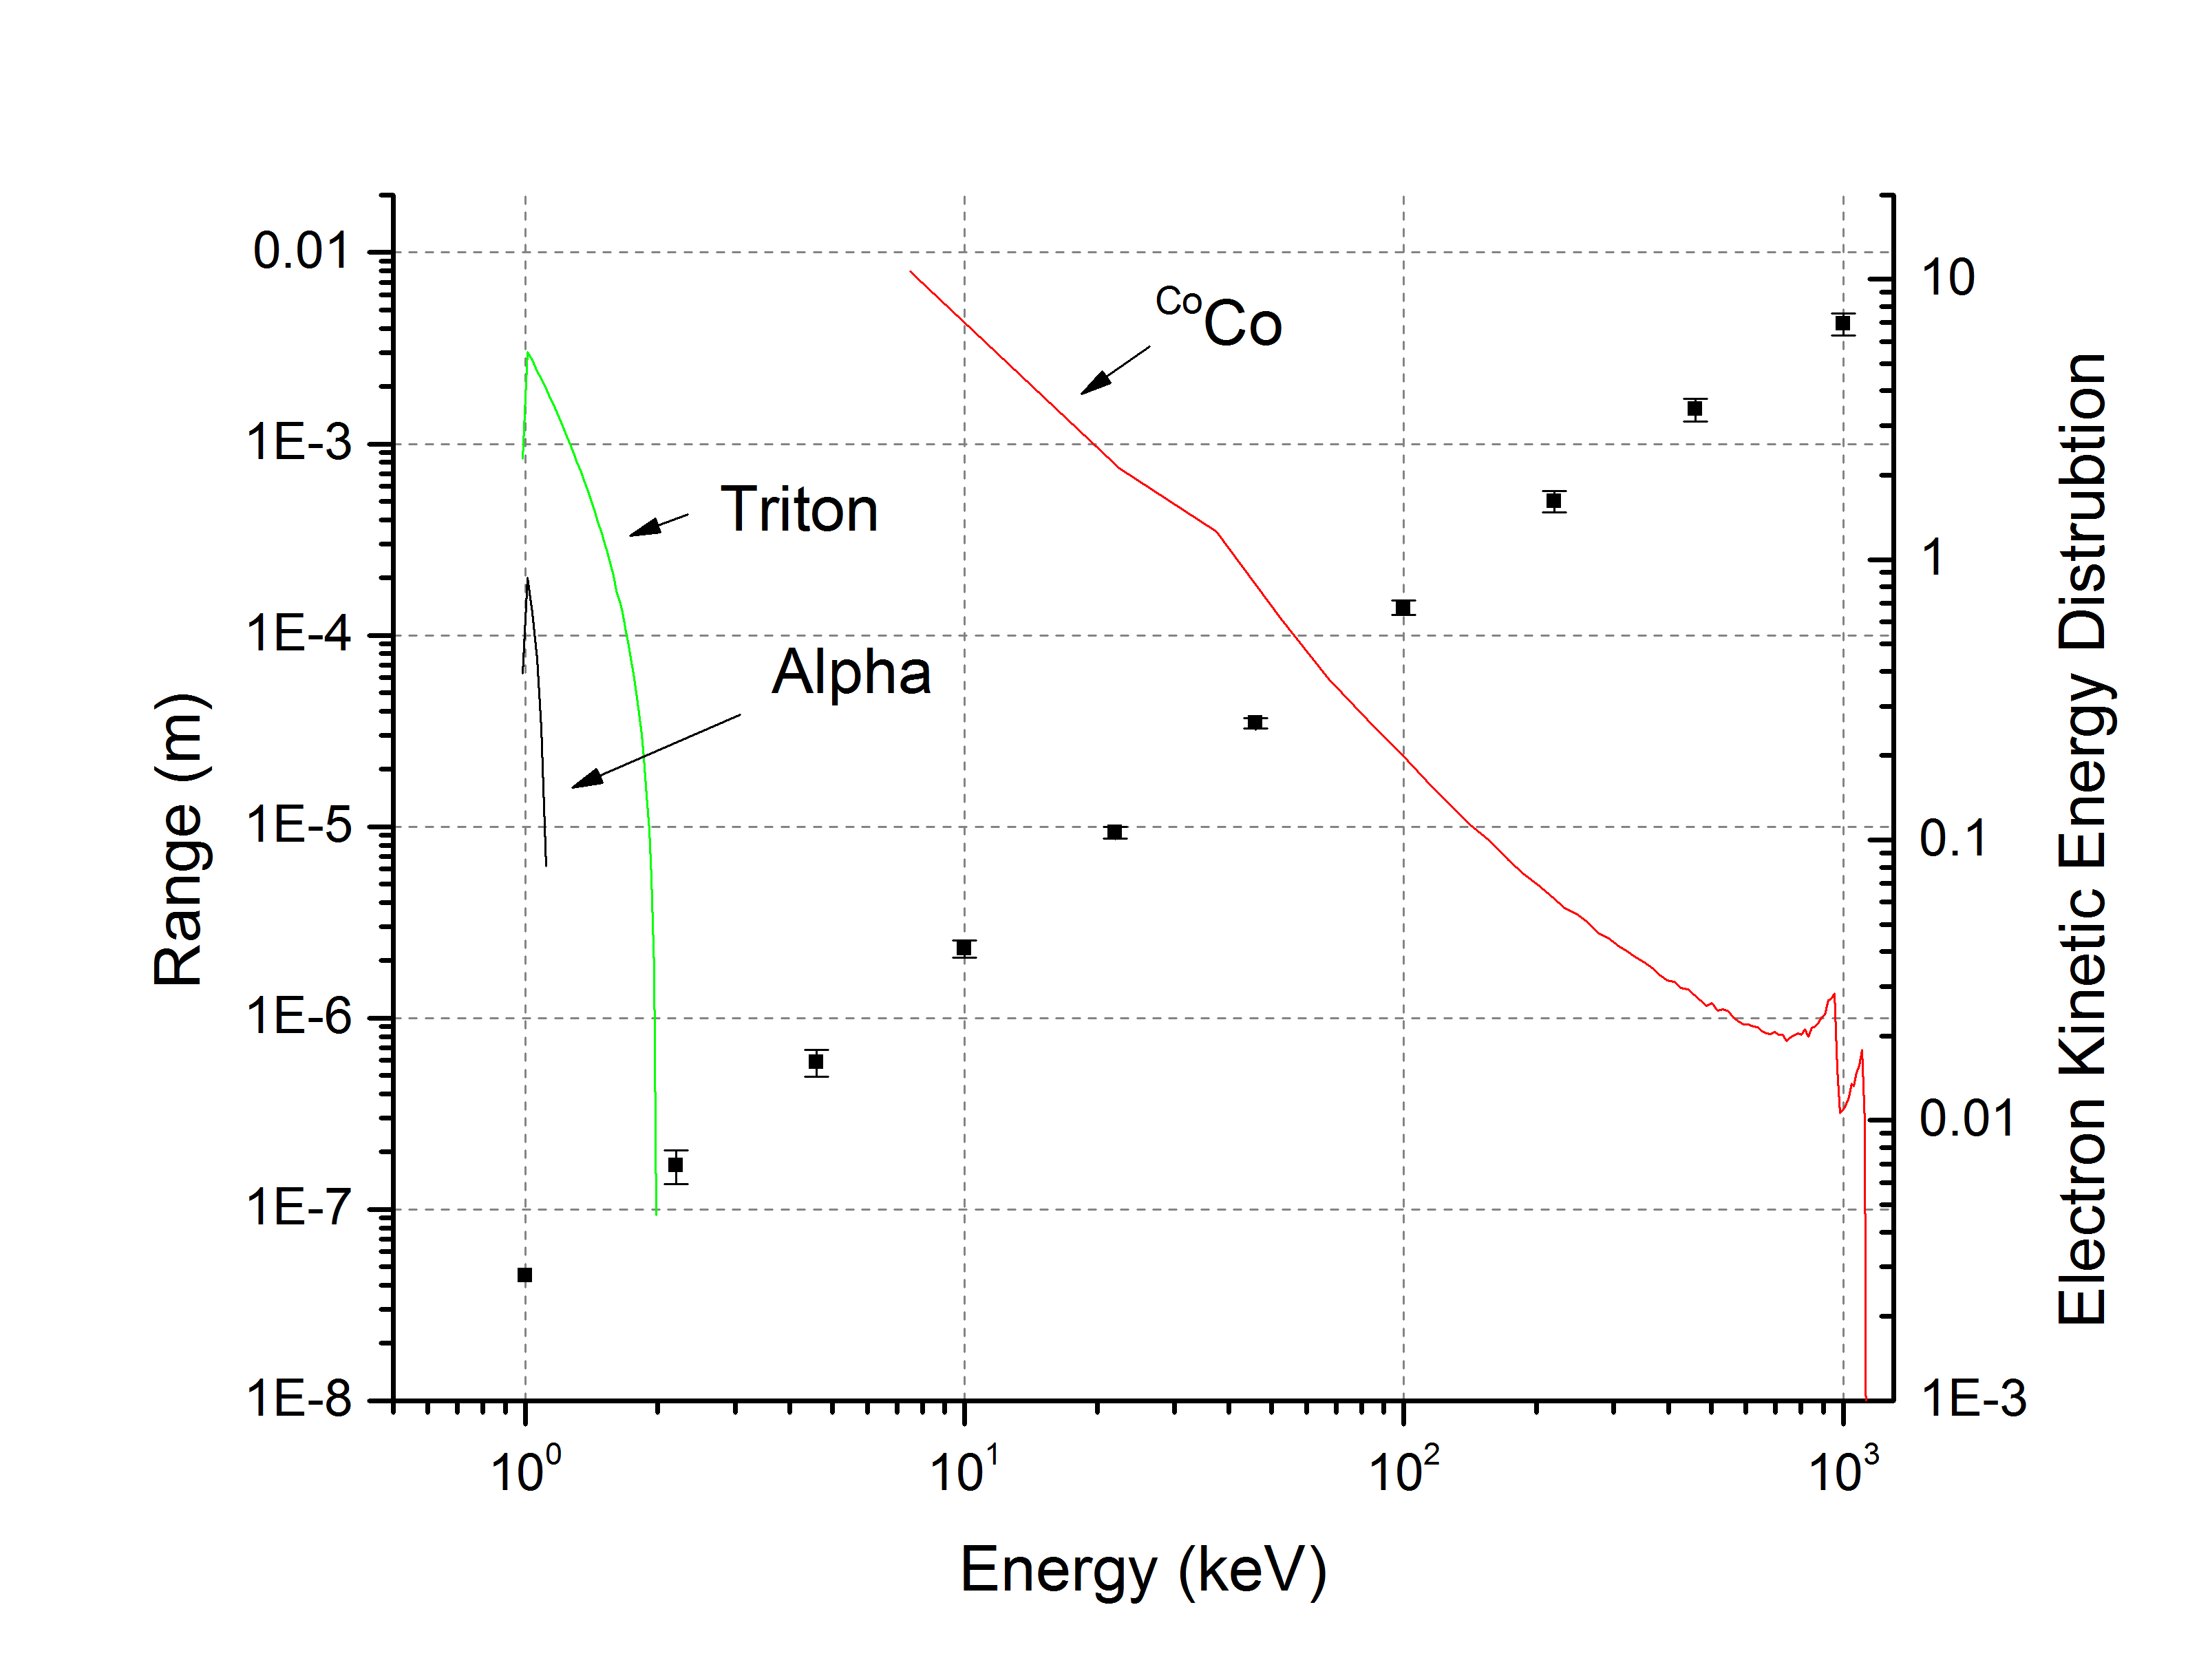
\includegraphics[width=\textwidth]{ElectronRangeAndEnergyDist}
  \caption[Electron Range and Energy Distribution of Selected Reactions]{The electron range corresponding to the square dots is shown on the left axis. The distribution of the kinetic energy of electrons from \SI{2.05}{\MeV} alpha, \SI{2.73}{\MeV} triton, and secondary electrons from \iso[60]{Co} are shown on the right. The \iso[60]{Co} electrons have energies much greater than the alpha and triton, and their corresponding range is orders of magnitude greater than the ranges of the electrons from the alpha and triton. For example, the average energy of a secondar electron has an kinetic energy around \SI{100}{\keV}, which corresponds to a range of \SI{0.1}{\mm}. \rangeSimGeo}
  \label{fig:ERangeAndDist}
\end{figure}
